\section{Concluding Remarks}
\label{sect:concluding_remarks}

In this thesis I have built a library for research and prototyping of algorithms in DSP/SDR topics, using free and open source technologies. The main objective has been to provide an initial framework as a stepping stone that can be extended in the future by fellow students and colleagues, with many other possible algorithms in these areas of research. The library has been developed in Python which is one of the most popular languages within the scientific community and enjoys a large array of mature supporting libraries for scientific use, such as \emph{NumPy}, \emph{SciPy} and \emph{Matplotlib}. The disadvantage is a performance penalty compared to compiled languages, but this has been deemed acceptable, given the goal is to focus on algorithm research and understanding (see \autoref{sect:future_investigation} for ways to move forward with respect to addressing performance concerns).

In addition to the library, I have demonstrated the use of GNU Radio as a framework for testing algorithms in real time and with hardware in the loop, which brings out a series of issues that cannot be ignored in real life applications. GNU Radio sometimes has a reputation for having a steep learning curve and lack of good documentation. While there is some truth to these claims, the fact is that it remains as a very flexible and interesting platform to develop SDR applications, once you take the time to understand its architecture. An impressive amount of technologies have been implemented in it, and many advanced algorithms and techniques are available such as polyphase fractional resamplers, to name one example. Like many other open source projects, sometimes you are required to dive into the source code and rely on the community, which is made of people who are not only very good DSP practitioners but, simultaneously, exceptional computer scientists and programmers, a very difficult combination to achieve, but which all engineers in this area should strive for.

\section{Summary of the work done}
\label{sect:summary_of_the_work_done}

First, a general introduction to SDR technologies has been written, with a brief historical background and surveys into the state of the art, both from the hardware and software perspectives.

Secondly a more detailed theoretical discussion of some of the more common SDR architectures was developed, with key advantages and disadvantages highlighted. To efficiently analyse and understand this discussion, one requires knowledge of basic RF and signal processing concepts and parameters. Towards this end a prior section was introduced, discussing some of these parameters, such as:
\begin{itemize}
  \item General concepts such as SNR, channel capacity (Shannon's formula) and $E_b/N_0$ to BER curves.
  \item ADC/DAC related metrics such as THD, SFDR, SINAD and ENOB.
  \item Impairments related to specific topologies such as IQ gain and phase offset for quadrature systems, and DC offset for ZIF systems.
\end{itemize}

After this, the proposed SKSDR library implementation was presented in detail. All developed algorithms were fully described from the theoretical point of view, and accompanied by usage examples in IPython and/or Jupyter notebooks.

Finally, the two proposed GNU Radio applications were described. An initial section was presented, with a more detailed look at the employed hardware (the HackRF One and the RTL-SDR) and an overview of GNU Radio architecture and flowgraph development. The remaining sections describe in detail each of the applications. An introduction to WBFM broadcast systems, in general, is made, describing the types of demodulating algorithms that exist. Following this, I make a description of the chosen algorithm for implementation, and a comparison it with the standard algorithm used by GNU Radio. An additional section describes the GR blocks developed for a PSK transceiver. These are mostly wrappers since the algorithm logic is mostly encapsulated in the SKSDR library. The developed complete transmitter and receiver flowgraphs making use of the GR blocks, are presented next, and its execution results both in conducted and radiated environment. Finally, a description is made about a new C++ module called \emph{Stream Demux} that was developed to separate an input stream into a number of output streams. This was needed to separate the preamble from the payload in the PSK receiver and, given it could have other uses in fixed packet size applications, submitted for integration to GNU Radio's codebase.

\section{Significant Results}
\label{sect:significant_results}

The key result is the creation of a library that can serve as a base for future prototyping and development of DSP/SDR algorithms, using only free and open source technologies. A significant effort was put into including a diverse set of algorithms which at this point already allow an end-to-end PSK transceiver system to function. This library has been developed with software best practices in mind, such as unit testing and documentation, so as to facilitate its future extensibility. In addition, several Jupyter notebooks were developed as proof of concept for individual modules of the library, and which simultaneously show, in general, the usefulness of the Jupyter framework for rapid prototyping.

Further, GNU Radio has been used to provide an engaging set of applications on top of the library, with real-time, actual hardware, and and over the air, specifications. This is important as it provides an alternative to simple simulation scenarios.

The proposed algorithm for alternate WBFM demodulation was successfully achieved with the performance being in good agreement with theory. This block could be used as a drop-in replacement for the GR standard WBFM Receiver block.

The PSK transceiver successfully demonstrates an end-to-end communication system using many of the important algorithms (especially on the receiver) developed. During the development an additional C++ GNU Radio block for stream demuxing was developed (specifically to separate the frame preamble from the payload) and which has been proposed for integration into GNU Radio codebase.

\section{Lessons Learned}
\label{sect:lessons_learnt}

Some of the most important takeaways obtained in the development of this thesis:
\begin{itemize}
  \item Ability to quickly put together a Python project with many of the software good practices in place is fairly easy to accomplish, given the extensive documentation available and maturity of the Python language.
  \item In-depth knowledge of the GNU Radio platform, its architecture, blocks and workflow development, becomes invaluable in the development of testing applications for SDR algorithms that can be applied with actual hardware and on existing systems. GR is not, however, the first tool of choice in the early stages of development, since its multi-threaded nature makes it more difficult to debug. For this reason, it's better to encapsulate the logic in a library, as it was done, and make use of unit testing and a debugger with stepping ability.
  \item Care must be taken to provide a library API that is efficient to use. For example, library modules should be able to take in a reference to an external buffer as argument instead of returning a self-created buffer. This reduces the amount of redundant data copying, a very expensive operation. For the same reason, scientific packages (\emph{NumPy} for example) should be used with caution. While they provide convenient APIs for many needed functionalities (correlation, filtering for example), these routines are often slow (because they are generic and have to work for many scenarios they implement lots of validations). A specific example is to avoid calling \code{np.hstack()} in loops, at all costs, which repeatedly copies data. Instead it's more efficient to use (whenever possible) one of the fast Python collection classes that implement common structures such as linked lists, queues and circular buffers.
  \item The use of Jupyter notebooks with its combined code, plotting and presentation capabilities, also facilitates early development, sharing or presentation of ideas, and collaboration (by using for example cloud Jupyter services such as Google Colab).
  \item In-depth knowledge of fundamental algorithms for digital receiver development such as synchronization techniques, which have wide application in almost every real system. This makes it much easier to understand and develop new applications (such as the suggestions in \autoref{sect:future_investigation}). Many of these techniques are based on PLLs and the detailed understanding of this theory will prove invaluable in future projects.
  \item Working with actual hardware in the loop introduces several issues which quite often deviate from simulated models. These can include buffer under/overflows in data processing, data type rounding and truncation issues (depending on the DSP platform used), multi-threading issues (in the case of a GPP SDR such as GNU Radio), real channel effects such as interference and fading which sometimes cannot be accurately captured in channel models, defective or malfunctioning hardware and/or connections that can cause frequency deviation, impedance mismatch, among other phenomena. For these reasons, it's very important to do extensive unit testing early on, that covers a large amount of use cases (even though it might seem a waste of time in the beginning, it will prove valuable in the long run).
  \item
\end{itemize}

\section{Future Investigation}
\label{sect:future_investigation}
There are many possible directions for future investigation. Here are a few suggestions:
\begin{itemize}
  \item Extending the library with other algorithms in the context of academic research. The more immediate candidates could be frequency modulation techniques such as the FSK family of modulations, specifically GMSK which is used in GSM communications.
  \item Re-implementing the available simple interpolator and decimator modules, using multirate techniques. Implementing a fractional resampler also.
  \item Other pulse-shaping techniques such as Gaussian filtering.
  \item Re-implementing some modules in C++ would make the performance in GNU Radio much better. These modules could be used by minimal wrapper GR blocks developed in C++ or even in Python (using the SWIG library which is what GNU Radio uses to call C++ from Python).
  \item Using the available modules for other projects. One example that was partially developed during the course of this thesis was the decoding of weather broadcasting satellites in LEO, such as the Meteor M2 satellite \cite{meteor_m2_sat} which uses QPSK. \autoref{fig:meteor_m2_flowgraph} shows a flowgraph for decoding Meteor M2's transmissions. Note that some of the modules already exist in the SKSDR library such as the interpolation/decimation, QPSK demodulator, AGC and RRC filtering. New modules would be the \emph{Costas Loop} for carrier synchronization (although perhaps the already developed phase/frequency synchronization module could achieve the same result) and the \emph{Mueller \& M{\"u}ller} clock recovery (again, could possibly be achieved with the already available symbol timing recovery module based on the ZCTED). Additional steps in fully decoding the signal (not shown in the flowgraph) include the implementation of Viterbi decoding, which would be a welcome addition to the library as a means to have a working implementation of convolutional error correcting codes.
\end{itemize}

\begin{figure}[ht]
  \centering
  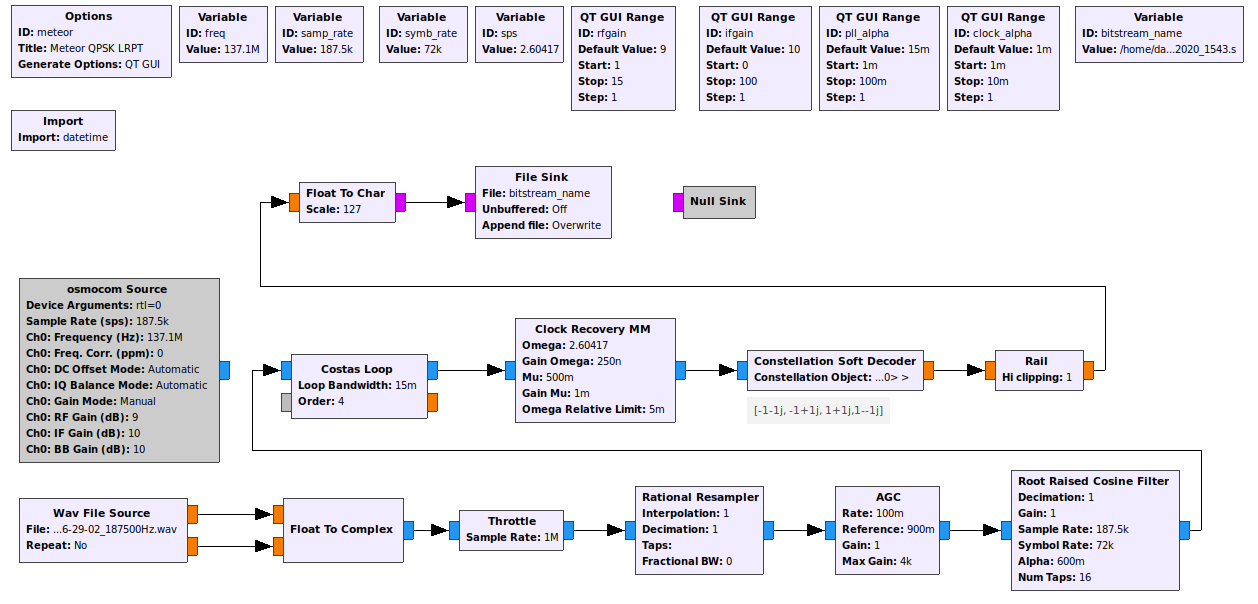
\includegraphics[width=\textwidth]{meteor_m2_flowgraph}
  \caption{A GNU Radio flowgraph for decoding Meteor M2 weather transmissions.}
  \label{fig:meteor_m2_flowgraph}
\end{figure}
